\chapter{Simulations and reconstructions}
\label{ch:reconstructions}


In order to develop and test reconstructions simulations are used. The in- and output are compared to test if the expected accuracy is achieved. Simulations are also used to better understand measured data, for example to test the effects of the Poisson distributed particle sampling and the detector response. First the simulations of the air showers which are the input for the detector simulation are described in the following section. Both Monte Carlo simulations of air showers and parametric approximations describing the time and density structures of the shower fronts are used.


\section{Monte Carlo extensive air shower simulation}

For the simulation of cosmic-ray induced air showers there are several programs available, most notably \corsika and \aires \cite{sciutto1999aires}. \corsika was chosen because development is still active, unlike \aires which received its last update in 2006. \corsika also includes updated models based on recent \lhc data. Additionally, \corsika is widely used by other cosmic-ray experiments.

\corsika version 74000 is used for all simulations reported in this thesis. \corsika provides the choice from many models for various interactions. For high energy hadronic interactions; DPMJET, EPOS \lhc \cite{pierog2013epos}, NEXUS, QGSJET, QGSJETII-04 \cite{ostapchenko2013qgsjetii}, SIBYLL, and VENUS are available. For hadrons with energies below \SI{80}{\GeV} GHEISHA \cite{fesefeldt1985}, FLUKA, or URQMD can be selected. Electromagnetic interactions can be treated by EGS4\cite{egs4} code or by NKG formulas.

From these options QGSJETII, GHEISHA and EGS4 were chosen. QGSJETII was chosen because the model has been tuned with \lhc data, and performs similar to EPOS, though both are not perfect yet (see ICRC2015 talks). Moreover, QGSJETII is easier to setup and faster to run [ref manual] than EPOS. All other options were left to their default values. The thinning algorithms were always disabled. For this configuration of \corsika an executable was compiled.  All simulations were performed using that same executable.

% From CORSIKA manual regarding model speed:
% - The QGSJETII04 option needs about 3 times more CPU-time than the HDPM  option (NKG enabled, EGS4 disabled).
% - The EPOS option needs roughly 7.5 times more CPU-time than the VENUS option (E0 = 1015 eV, NKG enabled, EGS4 disabled).
% - The VENUS option needs roughly 15 times more CPU-time than the HDPM option (NKG enabled, EGS4 disabled).
% So the EPOS option needs 7.5 x 15 = 112.5 times more CPU-time than the QGSJETII option. However, a large portion of simulation is not spent in the hadron models.


\subsection{Shower parameters}

The simulations are steered by an input file, most important parameters can be set here. The default options are used whenever applicable and believing in sensibly chosen defaults. The magnetic field and observation level values have been modified to values suitable for Amsterdam [ref]. The observation level for all simulations is set to\SI{10}{\meter} above sea level, which is relevant for the Science Park, where ground level is \SI{3.7}{\meter} below sea level, and the detector stations are on the roofs of buildings. The seeds for the random number generators (first for the hadron shower, second for EGS4) are randomly chosen and required to be unique for each simulation. The two seed values can be used as identifiers for specific simulations. Each combination of two seeds is unique in the dataset of simulations. A single air shower is simulated per run.

Each run is for a specific particle with a specific energy between \SIrange{e11}{e18}{\eV} in steps of $\log \frac{E}{\si{\eV}} = 0.5$. The zenith angle is also set for each run and is varied from\SIrange{0}{60}{\degree} in steps of \SI{7.5}{\degree}. The azimuthal angle is usually set to \SI{0}{\degree} (\hisparc coordinate system), but can be varied in steps of \SI{45}{\degree}.


\subsubsection{Primary particle}

Given the high abundance of protons as primary cosmic ray particles and iron with a relative high abundance for heavier nuclei these are the particles that were most focused on for the simulations. However, small datasets with other primaries have also been created. For protons all possible combinations of energy and zenith have been simulated at least 10 times. In \cref{fig:simulations_proton_energy_zenith} the number of simulated showers for each combination of the energy and zenith parameters for proton primaries can be seen. The focus was on the showers most often seen by \hisparc, i.e. primary energy of \SI{e15}{\eV} at \SI{22.5}{\degree} zenith.


\subsubsection{Energy cuts}

The \corsika simulations will be used as input for detector simulations. Therefore, if in the simulation particles are created which will not be detected by a \hisparc detector the particle can be ignored. In \corsika energy cuts can be set for different types of particles, as soon as particle of that type drop below that energy value they are no longer tracked in the simulation. The energy cuts have been set to \SI{300}{\MeV} for hadrons and muons, and \SI{3}{\MeV} for electrons and photons [ref LiO Tom]. Below these energies the particles will no longer produce significant signals in the detector and are quickly stopped/slowed by the atmosphere and decay [ref PDG, fig 28.5].


\subsection{Stoomboot}

To run a significant number of simulations the local \nikhef computer cluster 'Stoomboot' was utilized. This cluster used to have around 300 CPUs available, but was expanded in February 2014 to over 800 CPUs. Job queueing uses a fair-use policy to give each group at Nikhef equal opportunity to use computation time.

Simulation time for each simulation is different because the total number of particles in a shower will be different each run, even with the same starting paramters but with different seeds for the random number generators. Stoomboot has a maximum job time of \SI{96}{\hour}. This allows for showers with primary energies up to \SI{e17}{\eV}, which take around 60 hours to complete. Showers with primary energies less than \SI{e14}{\eV} are very quick and take only a minute [check] to complete. A large sample of showers can easily be generated by running many jobs simultaneously.

Cosmic rays with energies above \SI{e17}{\eV} have been observed, so some simulations at higher energies are desired. During the 2014 Christmas holidays 285 jobs at energies \SIlist{e17.5;e18}{\eV} were run. To allow this the maximum job time had been manually extended by a Stoomboot administrator. The longest jobs took over \SI{480}{\hour} (i.e.\SI{20}{\day}) to complete. In total over [check] \SI{50}{\year} of CPU time was used to generate the entire simulation sample.

\begin{figure}
    \centering
    % \usepackage{tikz}
% \usetikzlibrary{arrows,external}
% \usepackage{pgfplots}
% \pgfplotsset{compat=1.3}
% \usepackage[detect-family]{siunitx}
% \usepackage[eulergreek]{sansmath}
% \sisetup{text-sf=\sansmath}
% \usepackage{relsize}
%
    \tikzsetnextfilename{externalized-shower_walltime}
\pgfkeysifdefined{/artist/width}
    {\pgfkeysgetvalue{/artist/width}{\defaultwidth}}
    {\def\defaultwidth{ .67\linewidth }}
%
%
\begin{sansmath}
\begin{tikzpicture}[
        font=\sffamily,
        every pin/.style={inner sep=2pt, font={\sffamily\smaller}},
        every label/.style={inner sep=2pt, font={\sffamily\smaller}},
        every pin edge/.style={<-, >=stealth', shorten <=2pt},
        pin distance=2.5ex,
    ]
    \begin{axis}[
            axis background/.style={  },
            xmode=log,
            ymode=normal,
            width=\defaultwidth,
            scale only axis,
            axis equal=false,
            %
            title={  },
            %
            xlabel={ Walltime [\si{\hour}] },
            ylabel={ Count },
            %
            xmin={  },
            xmax={  },
            ymin={ 0 },
            ymax={  },
            %
            xtick={  },
            ytick={  },
            xticklabel style={  },
            yticklabel style={  },
            %
            tick align=outside,
            max space between ticks=40,
            every tick/.style={},
            axis on top,
            point meta min={  },
            point meta max={  },
                colormap={coolwarm}{
                    rgb255(0cm)=( 59, 76,192);
                    rgb255(1cm)=( 98,130,234);
                    rgb255(2cm)=(141,176,254);
                    rgb255(3cm)=(184,208,249);
                    rgb255(4cm)=(221,221,221);
                    rgb255(5cm)=(245,196,173);
                    rgb255(6cm)=(244,154,123);
                    rgb255(7cm)=(222, 96, 77);
                    rgb255(8cm)=(180,  4, 38)},
        ]

        


    
    % Draw series plot
    \addplot[no markers,solid,const plot] coordinates {
            (0.0036416653952, 871)
            (0.0038629679752, 1619)
            (0.00409771902632, 988)
            (0.0043467358069, 160)
            (0.00461088523971, 21)
            (0.00489108693012, 2)
            (0.00518831636753, 27)
            (0.00550360832145, 170)
            (0.00583806044395, 1064)
            (0.00619283709095, 1180)
            (0.00656917337587, 1068)
            (0.00696837946945, 691)
            (0.00739184516101, 299)
            (0.00784104469682, 257)
            (0.00831754191251, 528)
            (0.00882299567741, 744)
            (0.00935916566966, 776)
            (0.00992791850238, 704)
            (0.010531234222, 415)
            (0.0111712132017, 153)
            (0.0118500834533, 61)
            (0.0125702083843, 524)
            (0.0133340950254, 519)
            (0.0141444027585, 21)
            (0.0150039525752, 13)
            (0.0159157368977, 7)
            (0.0168829299964, 1)
            (0.017908899041, 2)
            (0.0189972158226, 0)
            (0.0201516691889, 1)
            (0.0213762782342, 0)
            (0.0226753062916, 0)
            (0.0240532757753, 1)
            (0.025514983925, 39)
            (0.0270655195065, 296)
            (0.0287102805281, 619)
            (0.030454993033, 433)
            (0.0323057310335, 368)
            (0.0342689376575, 586)
            (0.0363514475794, 956)
            (0.0385605108136, 1262)
            (0.0409038179556, 1110)
            (0.0433895269549, 1034)
            (0.0460262915167, 922)
            (0.0488232912284, 940)
            (0.0517902635173, 1149)
            (0.0549375375503, 1157)
            (0.0582760701939, 701)
            (0.0618174841588, 198)
            (0.0655741084636, 114)
            (0.0695590213562, 174)
            (0.0737860958449, 578)
            (0.078270047995, 63)
            (0.0830264881613, 564)
            (0.0880719753339, 34)
            (0.0934240747862, 0)
            (0.0991014192263, 4)
            (0.105123773665, 11)
            (0.111512104224, 55)
            (0.11828865113, 45)
            (0.125477006138, 43)
            (0.133102194664, 19)
            (0.141190762912, 10)
            (0.149770870284, 5)
            (0.158872387421, 0)
            (0.168527000191, 1)
            (0.178768319997, 1)
            (0.189632000798, 2)
            (0.201155863228, 1)
            (0.213380026264, 0)
            (0.226347046901, 1)
            (0.240102068304, 2)
            (0.254692976972, 7)
            (0.270170569445, 12)
            (0.286588729152, 211)
            (0.304004613995, 1348)
            (0.32247885534, 894)
            (0.342075769098, 583)
            (0.36286357963, 1590)
            (0.384914657267, 2904)
            (0.408305770258, 2482)
            (0.433118352025, 1230)
            (0.459438784669, 1041)
            (0.487358699699, 1421)
            (0.516975297031, 1443)
            (0.548391683386, 1264)
            (0.581717231236, 833)
            (0.617067959579, 543)
            (0.654566937841, 497)
            (0.694344714327, 75)
            (0.736539770713, 76)
            (0.781299004152, 262)
            (0.82877823868, 12)
            (0.879142767697, 1)
            (0.93256792942, 1)
            (0.989239717299, 0)
            (1.04935542754, 2)
            (1.11312434594, 4)
            (1.18076847655, 30)
            (1.25252331448, 87)
            (1.32863866582, 48)
            (1.40937951725, 9)
            (1.4950269586, 0)
            (1.58587916143, 2)
            (1.68225241704, 0)
            (1.78448223766, 1)
            (1.89292452445, 2)
            (2.00795680653, 2)
            (2.12997955535, 1)
            (2.25941757884, 0)
            (2.39672150032, 0)
            (2.54236932735, 1)
            (2.69686811578, 2)
            (2.86075573509, 7)
            (3.03460274085, 9)
            (3.21901436107, 37)
            (3.41463260323, 572)
            (3.62213848937, 3599)
            (3.84225442695, 1759)
            (4.07574672386, 1899)
            (4.32342825622, 1248)
            (4.5861612983, 954)
            (4.86486052447, 1215)
            (5.16049619348, 2520)
            (5.47409752632, 2001)
            (5.80675628935, 1315)
            (6.15963059515, 1420)
            (6.53394893432, 659)
            (6.93101445238, 103)
            (7.35220948648, 146)
            (7.79900037787, 50)
            (8.27294257677, 0)
            (8.77568605749, 0)
            (9.30898106267, 1)
            (9.87468419648, 0)
            (10.4747648882, 1)
            (11.1113122486, 5)
            (11.7865423427, 6)
            (12.5028059053, 25)
            (13.2625965241, 69)
            (14.0685593213, 24)
            (14.9235001621, 4)
            (15.8303954229, 1)
            (16.7924023536, 1)
            (17.8128700688, 3)
            (18.8953512074, 3)
            (20.0436143009, 6)
            (21.2616568929, 3)
            (22.5537194563, 4)
            (23.9243001557, 0)
            (25.3781705074, 1)
            (26.9203919912, 3)
            (28.5563336705, 1)
            (30.2916908851, 3)
            (32.132505078, 11)
            (34.0851848286, 16)
            (36.156528163, 47)
            (38.3537462206, 462)
            (40.6844883592, 1274)
            (43.1568687849, 1089)
            (45.7794948008, 866)
            (48.5614967727, 228)
            (51.5125599151, 145)
            (54.6429580089, 114)
            (57.9635891691, 120)
            (61.4860137845, 209)
            (65.2224947644, 168)
            (69.1860402303, 23)
            (73.390448802, 17)
            (77.8503576362, 14)
            (82.5812933837, 6)
            (87.5997262441, 0)
            (92.9231273041, 0)
            (98.5700293619, 0)
            (104.560091446, 0)
            (110.914167258, 0)
            (117.654377769, 4)
            (124.804188233, 9)
            (132.388489879, 35)
            (140.433686565, 47)
            (148.967786705, 4)
            (158.020500767, 0)
            (167.623344718, 0)
            (177.809749736, 0)
            (188.615178598, 0)
            (200.07724914, 0)
            (212.23586522, 0)
            (225.133355639, 0)
            (238.814621499, 0)
            (253.327292529, 0)
            (268.721892893, 0)
            (285.052017094, 0)
            (302.374516547, 0)
            (320.749697508, 0)
            (340.241531021, 2)
            (360.917875624, 4)
            (382.850713591, 5)
            (406.116401532, 51)
            (430.795936219, 70)
            (456.975236565, 44)
            (484.745442741, 44)
    };


    \end{axis}
\end{tikzpicture}
\end{sansmath}
    \caption{\captitle{Walltime for \corsika simulations.} Vertial lines indicate the walltime limits of the different Stoomboot queues.}
    \label{fig:simulations_shower_walltime}
\end{figure}


\subsection{No thinning}

% Explain how thinning helps to reduce computation time
% - Keep one particle if energy drops below fraction, only up to given weight
% - To reduce storage thin particles close to core at observation level
\corsika provides a thinning mechanism to reduce the computation time and storage requirements. This could allow for the simulation of even more energetic air showers, for cases where otherwise the simulation time would become unreasonable. Thinning works by taking particles emerging from interactions which are below a given fraction of the primary particle energy and drops all but one of those. The particle that is kept is given a weight to represent the number of dropped particles. These weights are then included with the particle information for the particles at the observation level. Additionally, particles close to the shower core at the observation level, where the detectors are likely saturated, may be thinned further to reduce the required storage size. The thinned shower output format is currently incompatible with the \hisparc detector simulation. The detector simulations requires individual particles, otherwise the particle density needs to be reconstructed to apply Poisson statistics to achieve the number of particles in a detector. A dethinning algorithm exists \cite{stokes2012} which can unravel the weighted particles into separate particles, of course some information is already lost.

% We do not use thinning because Stoomboot is fast enough for some 1e18 eV
The thinning mechanism has not been enabled because with Stoomboot enough computational time was available to run showers with energies up to \SI{e18}{\eV} without thinning. As shown by [LiO Sabine] the number of detected air showers by the Science Park cluster with primary energies above \SI{e18}{\eV} is low. Therefore simulated showers with higher energies are not immediately necessary, moreover, the extremely large file sizes make it harder to use them.


\subsection{Simulations catalogue}

Using Stoomboot a collection of over \num{70000} simulated showers has been created. This data, approximately \SI{20}{\tera\byte} [check], is stored on the \hisparc data server (trave) which has \SI{37}{\tera\byte} space. This space is shared with the raw \hisparc data (cosmic and weather), \knmi lightning data, and analysis files from various \hisparc collaborators.

For easy use with the \sapphire framework the \corsika simulations are converted from the sequential unformatted \fortran data format to \hdf format. This is done using a modified version of the the Python \corsika Reader package \cite{gonzalez2011}. During the conversion the values are (when applicable) converted to the units and coordinate systems used in \hisparc [see appendix].

After the initial conversion further optimisation is performed by sorting and indexing the 'x' coordinate column for the particles. In the detector simulation particles are queried from the \corsika data file using x and y coordinates. With the index it is very easy for the software to know which part of the data it needs. Since the data is sorted (on disk) only a small part of the data needs to be read into memory. If the data was not sorted more chunks of the file would need to be read into memory. In some cases the sorting speeds up simulations by a factor of 50 \cite{pytables:optimization}.

[TODO: Update plot with intermediate energies, and 'color bar', also one for iron?]

\begin{figure}
    \centering
    % \usepackage{tikz}
% \usetikzlibrary{arrows,external}
% \usepackage{pgfplots}
% \pgfplotsset{compat=1.3}
% \usepackage[detect-family]{siunitx}
% \usepackage[eulergreek]{sansmath}
% \sisetup{text-sf=\sansmath}
% \usepackage{relsize}
%
    \tikzsetnextfilename{externalized-energy_zenith_proton}
\pgfkeysifdefined{/artist/width}
    {\pgfkeysgetvalue{/artist/width}{\defaultwidth}}
    {\def\defaultwidth{ .67\linewidth }}
%
%
\begin{sansmath}
\begin{tikzpicture}[
        font=\sffamily,
        every pin/.style={inner sep=2pt, font={\sffamily\smaller}},
        every label/.style={inner sep=2pt, font={\sffamily\smaller}},
        every pin edge/.style={<-, >=stealth', shorten <=2pt},
        pin distance=2.5ex,
    ]
    \begin{axis}[
            axis background/.style={  },
            xmode=normal,
            ymode=normal,
            width=\defaultwidth,
            scale only axis,
            axis equal=false,
            %
            title={ Number of simulations per energy and zenith angle },
            %
            xlabel={ Energy [\si{electronvolt}] },
            ylabel={ Zenith [\si{\radian}] },
            %
            xmin={ 11.5 },
            xmax={ 19 },
            ymin={ -0.0654498 },
            ymax={ 1.11265 },
            %
            xtick={  },
            ytick={  },
            xticklabel style={  },
            yticklabel style={  },
            %
            tick align=outside,
            max space between ticks=40,
            every tick/.style={},
            axis on top,
            point meta min={  },
            point meta max={  },
                colormap={coolwarm}{
                    rgb255(0cm)=( 59, 76,192);
                    rgb255(1cm)=( 98,130,234);
                    rgb255(2cm)=(141,176,254);
                    rgb255(3cm)=(184,208,249);
                    rgb255(4cm)=(221,221,221);
                    rgb255(5cm)=(245,196,173);
                    rgb255(6cm)=(244,154,123);
                    rgb255(7cm)=(222, 96, 77);
                    rgb255(8cm)=(180,  4, 38)},
        ]

        
    % Draw histogram background, if needed

    % Draw non-empty bins in histogram
                    \draw[,
                          scale around={ 0.458703629157:
                                        (axis cs: 13.0, 0.0)}]
                        (axis cs:12.75, -0.0654498)
                        rectangle (axis cs:13.25, 0.0654498);
                    \draw[,
                          scale around={ 0.38726448431:
                                        (axis cs: 13.0, 0.1309)}]
                        (axis cs:12.75, 0.0654498)
                        rectangle (axis cs:13.25, 0.19635);
                    \draw[,
                          scale around={ 0.389290293168:
                                        (axis cs: 13.0, 0.261799)}]
                        (axis cs:12.75, 0.19635)
                        rectangle (axis cs:13.25, 0.327249);
                    \draw[,
                          scale around={ 0.45179244484:
                                        (axis cs: 13.0, 0.392699)}]
                        (axis cs:12.75, 0.327249)
                        rectangle (axis cs:13.25, 0.458149);
                    \draw[,
                          scale around={ 0.392643415327:
                                        (axis cs: 13.0, 0.523599)}]
                        (axis cs:12.75, 0.458149)
                        rectangle (axis cs:13.25, 0.589049);
                    \draw[,
                          scale around={ 0.378014019378:
                                        (axis cs: 13.0, 0.654498)}]
                        (axis cs:12.75, 0.589049)
                        rectangle (axis cs:13.25, 0.719948);
                    \draw[,
                          scale around={ 0.388616196916:
                                        (axis cs: 13.0, 0.785398)}]
                        (axis cs:12.75, 0.719948)
                        rectangle (axis cs:13.25, 0.850848);
                    \draw[,
                          scale around={ 0.161923415382:
                                        (axis cs: 13.0, 0.916298)}]
                        (axis cs:12.75, 0.850848)
                        rectangle (axis cs:13.25, 0.981748);
                    \draw[,
                          scale around={ 0.0809617076908:
                                        (axis cs: 13.0, 1.0472)}]
                        (axis cs:12.75, 0.981748)
                        rectangle (axis cs:13.25, 1.11265);
                    \draw[,
                          scale around={ 0.0362071763942:
                                        (axis cs: 13.5, 0.0)}]
                        (axis cs:13.25, -0.0654498)
                        rectangle (axis cs:13.75, 0.0654498);
                    \draw[,
                          scale around={ 0.0362071763942:
                                        (axis cs: 13.5, 0.1309)}]
                        (axis cs:13.25, 0.0654498)
                        rectangle (axis cs:13.75, 0.19635);
                    \draw[,
                          scale around={ 0.0362071763942:
                                        (axis cs: 13.5, 0.261799)}]
                        (axis cs:13.25, 0.19635)
                        rectangle (axis cs:13.75, 0.327249);
                    \draw[,
                          scale around={ 0.0379744069695:
                                        (axis cs: 13.5, 0.392699)}]
                        (axis cs:13.25, 0.327249)
                        rectangle (axis cs:13.75, 0.458149);
                    \draw[,
                          scale around={ 0.0362071763942:
                                        (axis cs: 13.5, 0.523599)}]
                        (axis cs:13.25, 0.458149)
                        rectangle (axis cs:13.75, 0.589049);
                    \draw[,
                          scale around={ 0.0362071763942:
                                        (axis cs: 13.5, 0.654498)}]
                        (axis cs:13.25, 0.589049)
                        rectangle (axis cs:13.75, 0.719948);
                    \draw[,
                          scale around={ 0.0362071763942:
                                        (axis cs: 13.5, 0.785398)}]
                        (axis cs:13.25, 0.719948)
                        rectangle (axis cs:13.75, 0.850848);
                    \draw[,
                          scale around={ 0.0362071763942:
                                        (axis cs: 13.5, 0.916298)}]
                        (axis cs:13.25, 0.850848)
                        rectangle (axis cs:13.75, 0.981748);
                    \draw[,
                          scale around={ 0.0362071763942:
                                        (axis cs: 13.5, 1.0472)}]
                        (axis cs:13.25, 0.981748)
                        rectangle (axis cs:13.75, 1.11265);
                    \draw[,
                          scale around={ 0.56033456932:
                                        (axis cs: 14.0, 0.0)}]
                        (axis cs:13.75, -0.0654498)
                        rectangle (axis cs:14.25, 0.0654498);
                    \draw[,
                          scale around={ 0.442705843146:
                                        (axis cs: 14.0, 0.1309)}]
                        (axis cs:13.75, 0.0654498)
                        rectangle (axis cs:14.25, 0.19635);
                    \draw[,
                          scale around={ 0.512686458081:
                                        (axis cs: 14.0, 0.261799)}]
                        (axis cs:13.75, 0.19635)
                        rectangle (axis cs:14.25, 0.327249);
                    \draw[,
                          scale around={ 0.56033456932:
                                        (axis cs: 14.0, 0.392699)}]
                        (axis cs:13.75, 0.327249)
                        rectangle (axis cs:14.25, 0.458149);
                    \draw[,
                          scale around={ 0.450048065952:
                                        (axis cs: 14.0, 0.523599)}]
                        (axis cs:13.75, 0.458149)
                        rectangle (axis cs:14.25, 0.589049);
                    \draw[,
                          scale around={ 0.442705843146:
                                        (axis cs: 14.0, 0.654498)}]
                        (axis cs:13.75, 0.589049)
                        rectangle (axis cs:14.25, 0.719948);
                    \draw[,
                          scale around={ 0.45367461988:
                                        (axis cs: 14.0, 0.785398)}]
                        (axis cs:13.75, 0.719948)
                        rectangle (axis cs:14.25, 0.850848);
                    \draw[,
                          scale around={ 0.181035881971:
                                        (axis cs: 14.0, 0.916298)}]
                        (axis cs:13.75, 0.850848)
                        rectangle (axis cs:14.25, 0.981748);
                    \draw[,
                          scale around={ 0.140229791188:
                                        (axis cs: 14.0, 1.0472)}]
                        (axis cs:13.75, 0.981748)
                        rectangle (axis cs:14.25, 1.11265);
                    \draw[,
                          scale around={ 0.051204679912:
                                        (axis cs: 14.5, 0.0)}]
                        (axis cs:14.25, -0.0654498)
                        rectangle (axis cs:14.75, 0.0654498);
                    \draw[,
                          scale around={ 0.051204679912:
                                        (axis cs: 14.5, 0.1309)}]
                        (axis cs:14.25, 0.0654498)
                        rectangle (axis cs:14.75, 0.19635);
                    \draw[,
                          scale around={ 0.051204679912:
                                        (axis cs: 14.5, 0.261799)}]
                        (axis cs:14.25, 0.19635)
                        rectangle (axis cs:14.75, 0.327249);
                    \draw[,
                          scale around={ 0.0627126691134:
                                        (axis cs: 14.5, 0.392699)}]
                        (axis cs:14.25, 0.327249)
                        rectangle (axis cs:14.75, 0.458149);
                    \draw[,
                          scale around={ 0.051204679912:
                                        (axis cs: 14.5, 0.523599)}]
                        (axis cs:14.25, 0.458149)
                        rectangle (axis cs:14.75, 0.589049);
                    \draw[,
                          scale around={ 0.051204679912:
                                        (axis cs: 14.5, 0.654498)}]
                        (axis cs:14.25, 0.589049)
                        rectangle (axis cs:14.75, 0.719948);
                    \draw[,
                          scale around={ 0.051204679912:
                                        (axis cs: 14.5, 0.785398)}]
                        (axis cs:14.25, 0.719948)
                        rectangle (axis cs:14.75, 0.850848);
                    \draw[,
                          scale around={ 0.051204679912:
                                        (axis cs: 14.5, 0.916298)}]
                        (axis cs:14.25, 0.850848)
                        rectangle (axis cs:14.75, 0.981748);
                    \draw[,
                          scale around={ 0.051204679912:
                                        (axis cs: 14.5, 1.0472)}]
                        (axis cs:14.25, 0.981748)
                        rectangle (axis cs:14.75, 1.11265);
                    \draw[,
                          scale around={ 0.702176554722:
                                        (axis cs: 15.0, 0.0)}]
                        (axis cs:14.75, -0.0654498)
                        rectangle (axis cs:15.25, 0.0654498);
                    \draw[,
                          scale around={ 0.497898046395:
                                        (axis cs: 15.0, 0.1309)}]
                        (axis cs:14.75, 0.0654498)
                        rectangle (axis cs:15.25, 0.19635);
                    \draw[,
                          scale around={ 0.605429030057:
                                        (axis cs: 15.0, 0.261799)}]
                        (axis cs:14.75, 0.19635)
                        rectangle (axis cs:15.25, 0.327249);
                    \draw[,
                          scale around={ 0.829215485849:
                                        (axis cs: 15.0, 0.392699)}]
                        (axis cs:14.75, 0.327249)
                        rectangle (axis cs:15.25, 0.458149);
                    \draw[,
                          scale around={ 0.447272219554:
                                        (axis cs: 15.0, 0.523599)}]
                        (axis cs:14.75, 0.458149)
                        rectangle (axis cs:15.25, 0.589049);
                    \draw[,
                          scale around={ 0.478839052256:
                                        (axis cs: 15.0, 0.654498)}]
                        (axis cs:14.75, 0.589049)
                        rectangle (axis cs:15.25, 0.719948);
                    \draw[,
                          scale around={ 0.461552747416:
                                        (axis cs: 15.0, 0.785398)}]
                        (axis cs:14.75, 0.719948)
                        rectangle (axis cs:15.25, 0.850848);
                    \draw[,
                          scale around={ 0.181035881971:
                                        (axis cs: 15.0, 0.916298)}]
                        (axis cs:14.75, 0.850848)
                        rectangle (axis cs:15.25, 0.981748);
                    \draw[,
                          scale around={ 0.120085618818:
                                        (axis cs: 15.0, 1.0472)}]
                        (axis cs:14.75, 0.981748)
                        rectangle (axis cs:15.25, 1.11265);
                    \draw[,
                          scale around={ 0.051204679912:
                                        (axis cs: 15.5, 0.0)}]
                        (axis cs:15.25, -0.0654498)
                        rectangle (axis cs:15.75, 0.0654498);
                    \draw[,
                          scale around={ 0.051204679912:
                                        (axis cs: 15.5, 0.1309)}]
                        (axis cs:15.25, 0.0654498)
                        rectangle (axis cs:15.75, 0.19635);
                    \draw[,
                          scale around={ 0.051204679912:
                                        (axis cs: 15.5, 0.261799)}]
                        (axis cs:15.25, 0.19635)
                        rectangle (axis cs:15.75, 0.327249);
                    \draw[,
                          scale around={ 0.051204679912:
                                        (axis cs: 15.5, 0.392699)}]
                        (axis cs:15.25, 0.327249)
                        rectangle (axis cs:15.75, 0.458149);
                    \draw[,
                          scale around={ 0.051204679912:
                                        (axis cs: 15.5, 0.523599)}]
                        (axis cs:15.25, 0.458149)
                        rectangle (axis cs:15.75, 0.589049);
                    \draw[,
                          scale around={ 0.051204679912:
                                        (axis cs: 15.5, 0.654498)}]
                        (axis cs:15.25, 0.589049)
                        rectangle (axis cs:15.75, 0.719948);
                    \draw[,
                          scale around={ 0.051204679912:
                                        (axis cs: 15.5, 0.785398)}]
                        (axis cs:15.25, 0.719948)
                        rectangle (axis cs:15.75, 0.850848);
                    \draw[,
                          scale around={ 0.051204679912:
                                        (axis cs: 15.5, 0.916298)}]
                        (axis cs:15.25, 0.850848)
                        rectangle (axis cs:15.75, 0.981748);
                    \draw[,
                          scale around={ 0.051204679912:
                                        (axis cs: 15.5, 1.0472)}]
                        (axis cs:15.25, 0.981748)
                        rectangle (axis cs:15.75, 1.11265);
                    \draw[,
                          scale around={ 0.68621913146:
                                        (axis cs: 16.0, 0.0)}]
                        (axis cs:15.75, -0.0654498)
                        rectangle (axis cs:16.25, 0.0654498);
                    \draw[,
                          scale around={ 0.410756014452:
                                        (axis cs: 16.0, 0.1309)}]
                        (axis cs:15.75, 0.0654498)
                        rectangle (axis cs:16.25, 0.19635);
                    \draw[,
                          scale around={ 0.469996485499:
                                        (axis cs: 16.0, 0.261799)}]
                        (axis cs:15.75, 0.19635)
                        rectangle (axis cs:16.25, 0.327249);
                    \draw[,
                          scale around={ 1.0:
                                        (axis cs: 16.0, 0.392699)}]
                        (axis cs:15.75, 0.327249)
                        rectangle (axis cs:16.25, 0.458149);
                    \draw[,
                          scale around={ 0.418345681938:
                                        (axis cs: 16.0, 0.523599)}]
                        (axis cs:15.75, 0.458149)
                        rectangle (axis cs:16.25, 0.589049);
                    \draw[,
                          scale around={ 0.436292719603:
                                        (axis cs: 16.0, 0.654498)}]
                        (axis cs:15.75, 0.589049)
                        rectangle (axis cs:16.25, 0.719948);
                    \draw[,
                          scale around={ 0.474852666688:
                                        (axis cs: 16.0, 0.785398)}]
                        (axis cs:15.75, 0.719948)
                        rectangle (axis cs:16.25, 0.850848);
                    \draw[,
                          scale around={ 0.22870786811:
                                        (axis cs: 16.0, 0.916298)}]
                        (axis cs:15.75, 0.850848)
                        rectangle (axis cs:16.25, 0.981748);
                    \draw[,
                          scale around={ 0.113923220909:
                                        (axis cs: 16.0, 1.0472)}]
                        (axis cs:15.75, 0.981748)
                        rectangle (axis cs:16.25, 1.11265);
                    \draw[,
                          scale around={ 0.0443445535964:
                                        (axis cs: 16.5, 0.0)}]
                        (axis cs:16.25, -0.0654498)
                        rectangle (axis cs:16.75, 0.0654498);
                    \draw[,
                          scale around={ 0.0443445535964:
                                        (axis cs: 16.5, 0.1309)}]
                        (axis cs:16.25, 0.0654498)
                        rectangle (axis cs:16.75, 0.19635);
                    \draw[,
                          scale around={ 0.0443445535964:
                                        (axis cs: 16.5, 0.261799)}]
                        (axis cs:16.25, 0.19635)
                        rectangle (axis cs:16.75, 0.327249);
                    \draw[,
                          scale around={ 0.0443445535964:
                                        (axis cs: 16.5, 0.392699)}]
                        (axis cs:16.25, 0.327249)
                        rectangle (axis cs:16.75, 0.458149);
                    \draw[,
                          scale around={ 0.0443445535964:
                                        (axis cs: 16.5, 0.523599)}]
                        (axis cs:16.25, 0.458149)
                        rectangle (axis cs:16.75, 0.589049);
                    \draw[,
                          scale around={ 0.0443445535964:
                                        (axis cs: 16.5, 0.654498)}]
                        (axis cs:16.25, 0.589049)
                        rectangle (axis cs:16.75, 0.719948);
                    \draw[,
                          scale around={ 0.0443445535964:
                                        (axis cs: 16.5, 0.785398)}]
                        (axis cs:16.25, 0.719948)
                        rectangle (axis cs:16.75, 0.850848);
                    \draw[,
                          scale around={ 0.0443445535964:
                                        (axis cs: 16.5, 0.916298)}]
                        (axis cs:16.25, 0.850848)
                        rectangle (axis cs:16.75, 0.981748);
                    \draw[,
                          scale around={ 0.0443445535964:
                                        (axis cs: 16.5, 1.0472)}]
                        (axis cs:16.25, 0.981748)
                        rectangle (axis cs:16.75, 1.11265);
                    \draw[,
                          scale around={ 0.287157378891:
                                        (axis cs: 17.0, 0.0)}]
                        (axis cs:16.75, -0.0654498)
                        rectangle (axis cs:17.25, 0.0654498);
                    \draw[,
                          scale around={ 0.240171237636:
                                        (axis cs: 17.0, 0.1309)}]
                        (axis cs:16.75, 0.0654498)
                        rectangle (axis cs:17.25, 0.19635);
                    \draw[,
                          scale around={ 0.264832663772:
                                        (axis cs: 17.0, 0.261799)}]
                        (axis cs:16.75, 0.19635)
                        rectangle (axis cs:17.25, 0.327249);
                    \draw[,
                          scale around={ 0.354386698156:
                                        (axis cs: 17.0, 0.392699)}]
                        (axis cs:16.75, 0.327249)
                        rectangle (axis cs:17.25, 0.458149);
                    \draw[,
                          scale around={ 0.263592222931:
                                        (axis cs: 17.0, 0.523599)}]
                        (axis cs:16.75, 0.458149)
                        rectangle (axis cs:17.25, 0.589049);
                    \draw[,
                          scale around={ 0.210188818153:
                                        (axis cs: 17.0, 0.654498)}]
                        (axis cs:16.75, 0.589049)
                        rectangle (axis cs:17.25, 0.719948);
                    \draw[,
                          scale around={ 0.305087091162:
                                        (axis cs: 17.0, 0.785398)}]
                        (axis cs:16.75, 0.719948)
                        rectangle (axis cs:17.25, 0.850848);
                    \draw[,
                          scale around={ 0.18813800734:
                                        (axis cs: 17.0, 0.916298)}]
                        (axis cs:16.75, 0.850848)
                        rectangle (axis cs:17.25, 0.981748);
                    \draw[,
                          scale around={ 0.125425338227:
                                        (axis cs: 17.0, 1.0472)}]
                        (axis cs:16.75, 0.981748)
                        rectangle (axis cs:17.25, 1.11265);
                    \draw[,
                          scale around={ 0.0198314872547:
                                        (axis cs: 17.5, 0.261799)}]
                        (axis cs:17.25, 0.19635)
                        rectangle (axis cs:17.75, 0.327249);
                    \draw[,
                          scale around={ 0.0302930971627:
                                        (axis cs: 17.5, 0.392699)}]
                        (axis cs:17.25, 0.327249)
                        rectangle (axis cs:17.75, 0.458149);
                    \draw[,
                          scale around={ 0.0302930971627:
                                        (axis cs: 17.5, 0.523599)}]
                        (axis cs:17.25, 0.458149)
                        rectangle (axis cs:17.75, 0.589049);
                    \draw[,
                          scale around={ 0.0362071763942:
                                        (axis cs: 17.5, 0.654498)}]
                        (axis cs:17.25, 0.589049)
                        rectangle (axis cs:17.75, 0.719948);
                    \draw[,
                          scale around={ 0.0443445535964:
                                        (axis cs: 17.5, 0.785398)}]
                        (axis cs:17.25, 0.719948)
                        rectangle (axis cs:17.75, 0.850848);
                    \draw[,
                          scale around={ 0.0362071763942:
                                        (axis cs: 17.5, 0.916298)}]
                        (axis cs:17.25, 0.850848)
                        rectangle (axis cs:17.75, 0.981748);
                    \draw[,
                          scale around={ 0.0343491435148:
                                        (axis cs: 17.5, 1.0472)}]
                        (axis cs:17.25, 0.981748)
                        rectangle (axis cs:17.75, 1.11265);
                    \draw[,
                          scale around={ 0.0362071763942:
                                        (axis cs: 18.0, 0.654498)}]
                        (axis cs:17.75, 0.589049)
                        rectangle (axis cs:18.25, 0.719948);
                    \draw[,
                          scale around={ 0.0412825327369:
                                        (axis cs: 18.0, 0.785398)}]
                        (axis cs:17.75, 0.719948)
                        rectangle (axis cs:18.25, 0.850848);
                    \draw[,
                          scale around={ 0.0443445535964:
                                        (axis cs: 18.0, 0.916298)}]
                        (axis cs:17.75, 0.850848)
                        rectangle (axis cs:18.25, 0.981748);
                    \draw[,
                          scale around={ 0.0443445535964:
                                        (axis cs: 18.0, 1.0472)}]
                        (axis cs:17.75, 0.981748)
                        rectangle (axis cs:18.25, 1.11265);




    \end{axis}
\end{tikzpicture}
\end{sansmath}
    \caption{\captitle{Proton simulations overview.} The square of the area of the rectangles indicate the number simulations with that energy and zenithb combinations with a proton primary.}
    \label{fig:simulations_proton_energy_zenith}
\end{figure}


\subsubsection{Simulation overview}

Whenever new simulations are performed they are automatically converted to \hdf and added to an overview. The overview can for instance be used to find a suitable \corsika simulation for a detector simulation. The overview contains the variable input parameters, the number of particles on ground level per particle type, and the height of first interaction for each simulation. From this data we can compare the shower sizes for proton primary showers as a function of energy and zenith angle. The shower sizes, in this case the sum of all leptons, are shown in \cref{fig:simulations_shower_sizes}. There is a clear separation between the shower sizes for particle of different energies, in steps of $\log(\frac{E}{\si{eV}}$, at the same inclination. There may be some overlap between showers of adjacent energies, but only at the few percentile level.

\begin{figure}
    \centering
    % \usepackage{tikz}
% \usetikzlibrary{arrows,external}
% \usepackage{pgfplots}
% \pgfplotsset{compat=1.3}
% \usepackage[detect-family]{siunitx}
% \usepackage[eulergreek]{sansmath}
% \sisetup{text-sf=\sansmath}
% \usepackage{relsize}
%
    \tikzsetnextfilename{externalized-shower_sizes}
\pgfkeysifdefined{/artist/width}
    {\pgfkeysgetvalue{/artist/width}{\defaultwidth}}
    {\def\defaultwidth{ .67\linewidth }}
%
%
\begin{sansmath}
\begin{tikzpicture}[
        font=\sffamily,
        every pin/.style={inner sep=2pt, font={\sffamily\smaller}},
        every label/.style={inner sep=2pt, font={\sffamily\smaller}},
        every pin edge/.style={<-, >=stealth', shorten <=2pt},
        pin distance=2.5ex,
    ]
    \begin{axis}[
            axis background/.style={  },
            xmode=normal,
            ymode=log,
            width=\defaultwidth,
            scale only axis,
            axis equal=false,
            %
            title={  },
            %
            xlabel={ Zenith [\si{\radian}] },
            ylabel={ Shower size (leptons) },
            %
            xmin={  },
            xmax={  },
            ymin={  },
            ymax={  },
            %
            xtick={  },
            ytick={  },
            xticklabel style={  },
            yticklabel style={  },
            %
            tick align=outside,
            max space between ticks=40,
            every tick/.style={},
            axis on top,
            point meta min={  },
            point meta max={  },
                colormap={coolwarm}{
                    rgb255(0cm)=( 59, 76,192);
                    rgb255(1cm)=( 98,130,234);
                    rgb255(2cm)=(141,176,254);
                    rgb255(3cm)=(184,208,249);
                    rgb255(4cm)=(221,221,221);
                    rgb255(5cm)=(245,196,173);
                    rgb255(6cm)=(244,154,123);
                    rgb255(7cm)=(222, 96, 77);
                    rgb255(8cm)=(180,  4, 38)},
        ]

        


    \addplot[draw=none, fill=lightgray,semitransparent] coordinates {
            (0.0, 11382.32)
            (0.1309, 11341.72)
            (0.261799, 12438.0)
            (0.392699, 8049.92)
            (0.523599, 7857.68)
            (0.654498, 4526.32)
            (0.785398, 2570.32)
            (0.916298, 1866.2)
            (1.0472, 1255.32)
            (1.0472, 2253.52)
            (0.916298, 2965.04)
            (0.785398, 5894.72)
            (0.654498, 10405.0)
            (0.523599, 19943.2)
            (0.392699, 24771.12)
            (0.261799, 24461.44)
            (0.1309, 37076.92)
            (0.0, 47313.76)
            } -- cycle;

    \addplot[draw=none, fill=lightgray,semitransparent] coordinates {
            (0.0, 631.2)
            (0.1309, 657.56)
            (0.261799, 630.88)
            (0.392699, 324.8)
            (0.523599, 476.44)
            (0.654498, 407.76)
            (0.785398, 309.36)
            (0.916298, 273.8)
            (1.0472, 163.88)
            (1.0472, 319.0)
            (0.916298, 409.44)
            (0.785398, 351.36)
            (0.654498, 595.0)
            (0.523599, 1162.96)
            (0.392699, 1067.2)
            (0.261799, 1698.84)
            (0.1309, 1989.32)
            (0.0, 1668.52)
            } -- cycle;

    \addplot[draw=none, fill=lightgray,semitransparent] coordinates {
            (0.261799, 37247828.0)
            (0.392699, 34000685.76)
            (0.523599, 22196393.76)
            (0.654498, 12001765.76)
            (0.785398, 5201100.2)
            (0.916298, 1779225.68)
            (1.0472, 906333.52)
            (1.0472, 1328089.76)
            (0.916298, 3738917.72)
            (0.785398, 8480915.2)
            (0.654498, 20569885.92)
            (0.523599, 29420888.16)
            (0.392699, 43290873.6)
            (0.261799, 40378553.44)
            } -- cycle;

    \addplot[draw=none, fill=lightgray,semitransparent] coordinates {
            (0.0, 199062.44)
            (0.1309, 184078.96)
            (0.261799, 186163.28)
            (0.392699, 123920.2)
            (0.523599, 88336.24)
            (0.654498, 64867.0)
            (0.785398, 29158.6)
            (0.916298, 17920.52)
            (1.0472, 14137.32)
            (1.0472, 17985.36)
            (0.916298, 35205.68)
            (0.785398, 60415.96)
            (0.654498, 253588.08)
            (0.523599, 208427.92)
            (0.392699, 404007.56)
            (0.261799, 327410.48)
            (0.1309, 460465.32)
            (0.0, 510995.56)
            } -- cycle;

    \addplot[draw=none, fill=lightgray,semitransparent] coordinates {
            (0.0, 16.0)
            (0.1309, 16.0)
            (0.261799, 16.0)
            (0.392699, 14.0)
            (0.523599, 14.0)
            (0.654498, 13.0)
            (0.785398, 11.0)
            (0.916298, 8.84)
            (0.916298, 19.16)
            (0.785398, 23.16)
            (0.654498, 27.0)
            (0.523599, 31.0)
            (0.392699, 35.0)
            (0.261799, 38.16)
            (0.1309, 44.16)
            (0.0, 48.0)
            } -- cycle;

    \addplot[draw=none, fill=lightgray,semitransparent] coordinates {
            (0.0, 169.0)
            (0.1309, 182.0)
            (0.261799, 146.24)
            (0.392699, 132.0)
            (0.523599, 118.0)
            (0.654498, 101.24)
            (0.785398, 83.0)
            (0.916298, 70.84)
            (1.0472, 66.68)
            (1.0472, 116.32)
            (0.916298, 135.48)
            (0.785398, 167.76)
            (0.654498, 226.52)
            (0.523599, 341.76)
            (0.392699, 414.52)
            (0.261799, 518.8)
            (0.1309, 639.16)
            (0.0, 609.76)
            } -- cycle;

    \addplot[draw=none, fill=lightgray,semitransparent] coordinates {
            (0.0, 2853.4)
            (0.1309, 2701.16)
            (0.261799, 2350.12)
            (0.392699, 1798.44)
            (0.523599, 1451.12)
            (0.654498, 1028.0)
            (0.785398, 807.72)
            (0.916298, 662.04)
            (1.0472, 536.68)
            (1.0472, 788.16)
            (0.916298, 1092.96)
            (0.785398, 1698.84)
            (0.654498, 2903.76)
            (0.523599, 5344.28)
            (0.392699, 6860.12)
            (0.261799, 9083.84)
            (0.1309, 9761.56)
            (0.0, 10130.64)
            } -- cycle;

    \addplot[draw=none, fill=lightgray,semitransparent] coordinates {
            (0.0, 55136.12)
            (0.1309, 51547.4)
            (0.261799, 44947.24)
            (0.392699, 33723.4)
            (0.523599, 22061.84)
            (0.654498, 13799.28)
            (0.785398, 8706.2)
            (0.916298, 5919.8)
            (1.0472, 4005.12)
            (1.0472, 6357.6)
            (0.916298, 10099.68)
            (0.785398, 20933.92)
            (0.654498, 38118.72)
            (0.523599, 68579.56)
            (0.392699, 101335.0)
            (0.261799, 133711.68)
            (0.1309, 151807.64)
            (0.0, 166450.84)
            } -- cycle;

    \addplot[draw=none, fill=lightgray,semitransparent] coordinates {
            (0.0, 933444.84)
            (0.1309, 890634.36)
            (0.261799, 755564.88)
            (0.392699, 569171.24)
            (0.523599, 369110.8)
            (0.654498, 200854.24)
            (0.785398, 101316.6)
            (0.916298, 56003.6)
            (1.0472, 34741.2)
            (1.0472, 51160.28)
            (0.916298, 97492.36)
            (0.785398, 219722.8)
            (0.654498, 537116.16)
            (0.523599, 930104.2)
            (0.392699, 1412316.92)
            (0.261799, 1861482.28)
            (0.1309, 1999034.92)
            (0.0, 2168503.84)
            } -- cycle;

    \addplot[draw=none, fill=lightgray,semitransparent] coordinates {
            (0.0, 14051766.36)
            (0.1309, 13798365.0)
            (0.261799, 11654958.8)
            (0.392699, 8740413.16)
            (0.523599, 5463975.44)
            (0.654498, 2883176.16)
            (0.785398, 1286342.76)
            (0.916298, 575788.4)
            (1.0472, 327520.4)
            (1.0472, 447841.64)
            (0.916298, 973584.76)
            (0.785398, 2886783.12)
            (0.654498, 7839064.24)
            (0.523599, 12967109.12)
            (0.392699, 17937112.08)
            (0.261799, 25781858.0)
            (0.1309, 26230808.0)
            (0.0, 28442164.8)
            } -- cycle;

    \addplot[draw=none, fill=lightgray,semitransparent] coordinates {
            (0.654498, 36715305.92)
            (0.785398, 16066389.36)
            (0.916298, 6209193.56)
            (1.0472, 3079834.76)
            (1.0472, 3563681.28)
            (0.916298, 10707477.12)
            (0.785398, 23453379.2)
            (0.654498, 40468008.96)
            } -- cycle;

    \addplot[draw=none, fill=lightgray,semitransparent] coordinates {
            (0.0, 3432960.72)
            (0.1309, 3390485.4)
            (0.261799, 3053419.24)
            (0.392699, 2867473.28)
            (0.523599, 1442700.56)
            (0.654498, 776463.32)
            (0.785398, 343483.36)
            (0.916298, 176362.04)
            (1.0472, 98726.44)
            (1.0472, 152729.32)
            (0.916298, 292981.96)
            (0.785398, 752531.56)
            (0.654498, 2502825.92)
            (0.523599, 3601883.96)
            (0.392699, 4744789.04)
            (0.261799, 7158101.84)
            (0.1309, 7388482.2)
            (0.0, 9846644.96)
            } -- cycle;

    
    % Draw series plot
    \addplot[mark=*,mark options=white,only marks] coordinates {
            (0.0, 4.37281e+06)
            (0.1309, 5.4088e+06)
            (0.261799, 4.89299e+06)
            (0.392699, 3.38686e+06)
            (0.523599, 1.84289e+06)
            (0.654498, 1.23085e+06)
            (0.785398, 582579.0)
            (0.916298, 199512.0)
            (1.0472, 130062.0)
    };

    
    % Draw series plot
    \addplot[mark=*,mark options=white,only marks] coordinates {
            (0.654498, 4.01265e+07)
            (0.785398, 2.00544e+07)
            (0.916298, 7.93248e+06)
            (1.0472, 3.25808e+06)
    };

    
    % Draw series plot
    \addplot[mark=*,mark options=white,only marks] coordinates {
            (0.0, 1.87288e+07)
            (0.1309, 1.73035e+07)
            (0.261799, 1.59842e+07)
            (0.392699, 1.18518e+07)
            (0.523599, 7.70421e+06)
            (0.654498, 4.46561e+06)
            (0.785398, 1.73332e+06)
            (0.916298, 713648.0)
            (1.0472, 393638.0)
    };

    
    % Draw series plot
    \addplot[mark=*,mark options=white,only marks] coordinates {
            (0.0, 1.33579e+06)
            (0.1309, 1.27176e+06)
            (0.261799, 1.09588e+06)
            (0.392699, 834848.0)
            (0.523599, 549684.0)
            (0.654498, 305770.0)
            (0.785398, 137276.0)
            (0.916298, 69467.0)
            (1.0472, 43057.0)
    };

    
    % Draw series plot
    \addplot[mark=*,mark options=white,only marks] coordinates {
            (0.0, 88484.0)
            (0.1309, 81400.0)
            (0.261799, 72721.5)
            (0.392699, 54856.0)
            (0.523599, 36047.5)
            (0.654498, 21661.0)
            (0.785398, 11874.0)
            (0.916298, 7790.0)
            (1.0472, 5226.5)
    };

    
    % Draw series plot
    \addplot[mark=*,mark options=white,only marks] coordinates {
            (0.0, 5043.5)
            (0.1309, 5117.5)
            (0.261799, 4144.0)
            (0.392699, 3174.5)
            (0.523599, 2407.5)
            (0.654498, 1555.5)
            (0.785398, 1110.0)
            (0.916298, 863.0)
            (1.0472, 658.5)
    };

    
    % Draw series plot
    \addplot[mark=*,mark options=white,only marks] coordinates {
            (0.0, 287.0)
            (0.1309, 299.0)
            (0.261799, 248.0)
            (0.392699, 209.0)
            (0.523599, 188.0)
            (0.654498, 149.5)
            (0.785398, 120.0)
            (0.916298, 97.0)
            (1.0472, 82.5)
    };

    
    % Draw series plot
    \addplot[mark=*,mark options=white,only marks] coordinates {
            (0.0, 28.5)
            (0.1309, 26.0)
            (0.261799, 24.0)
            (0.392699, 22.0)
            (0.523599, 21.0)
            (0.654498, 19.0)
            (0.785398, 17.0)
            (0.916298, 13.0)
    };

    
    % Draw series plot
    \addplot[mark=*,mark options=white,only marks] coordinates {
            (0.0, 383208.0)
            (0.1309, 312196.0)
            (0.261799, 268031.0)
            (0.392699, 210422.0)
            (0.523599, 135921.0)
            (0.654498, 118724.0)
            (0.785398, 42832.5)
            (0.916298, 23830.0)
            (1.0472, 15279.0)
    };

    
    % Draw series plot
    \addplot[mark=*,mark options=white,only marks] coordinates {
            (0.261799, 3.95884e+07)
            (0.392699, 3.87502e+07)
            (0.523599, 2.62175e+07)
            (0.654498, 1.5439e+07)
            (0.785398, 6.37078e+06)
            (0.916298, 2.50866e+06)
            (1.0472, 1.1277e+06)
    };

    
    % Draw series plot
    \addplot[mark=*,mark options=white,only marks] coordinates {
            (0.0, 1174.5)
            (0.1309, 1347.5)
            (0.261799, 1035.5)
            (0.392699, 658.0)
            (0.523599, 544.5)
            (0.654498, 520.5)
            (0.785398, 329.5)
            (0.916298, 355.5)
            (1.0472, 234.5)
    };

    
    % Draw series plot
    \addplot[mark=*,mark options=white,only marks] coordinates {
            (0.0, 14349.0)
            (0.1309, 17555.0)
            (0.261799, 19999.5)
            (0.392699, 12572.0)
            (0.523599, 11831.5)
            (0.654498, 6237.0)
            (0.785398, 3536.0)
            (0.916298, 2383.5)
            (1.0472, 1750.0)
    };

    
    % Draw series plot
    \addplot[mark=o,solid] coordinates {
            (0.0, 14349.0)
            (0.1309, 17555.0)
            (0.261799, 19999.5)
            (0.392699, 12572.0)
            (0.523599, 11831.5)
            (0.654498, 6237.0)
            (0.785398, 3536.0)
            (0.916298, 2383.5)
            (1.0472, 1750.0)
    };

    
    % Draw series plot
    \addplot[mark=o,solid] coordinates {
            (0.0, 1174.5)
            (0.1309, 1347.5)
            (0.261799, 1035.5)
            (0.392699, 658.0)
            (0.523599, 544.5)
            (0.654498, 520.5)
            (0.785398, 329.5)
            (0.916298, 355.5)
            (1.0472, 234.5)
    };

    
    % Draw series plot
    \addplot[mark=o,solid] coordinates {
            (0.261799, 3.95884e+07)
            (0.392699, 3.87502e+07)
            (0.523599, 2.62175e+07)
            (0.654498, 1.5439e+07)
            (0.785398, 6.37078e+06)
            (0.916298, 2.50866e+06)
            (1.0472, 1.1277e+06)
    };

    
    % Draw series plot
    \addplot[mark=o,solid] coordinates {
            (0.0, 383208.0)
            (0.1309, 312196.0)
            (0.261799, 268031.0)
            (0.392699, 210422.0)
            (0.523599, 135921.0)
            (0.654498, 118724.0)
            (0.785398, 42832.5)
            (0.916298, 23830.0)
            (1.0472, 15279.0)
    };

    
    % Draw series plot
    \addplot[mark=o,solid] coordinates {
            (0.0, 28.5)
            (0.1309, 26.0)
            (0.261799, 24.0)
            (0.392699, 22.0)
            (0.523599, 21.0)
            (0.654498, 19.0)
            (0.785398, 17.0)
            (0.916298, 13.0)
    };

    
    % Draw series plot
    \addplot[mark=o,solid] coordinates {
            (0.0, 287.0)
            (0.1309, 299.0)
            (0.261799, 248.0)
            (0.392699, 209.0)
            (0.523599, 188.0)
            (0.654498, 149.5)
            (0.785398, 120.0)
            (0.916298, 97.0)
            (1.0472, 82.5)
    };

    
    % Draw series plot
    \addplot[mark=o,solid] coordinates {
            (0.0, 5043.5)
            (0.1309, 5117.5)
            (0.261799, 4144.0)
            (0.392699, 3174.5)
            (0.523599, 2407.5)
            (0.654498, 1555.5)
            (0.785398, 1110.0)
            (0.916298, 863.0)
            (1.0472, 658.5)
    };

    
    % Draw series plot
    \addplot[mark=o,solid] coordinates {
            (0.0, 88484.0)
            (0.1309, 81400.0)
            (0.261799, 72721.5)
            (0.392699, 54856.0)
            (0.523599, 36047.5)
            (0.654498, 21661.0)
            (0.785398, 11874.0)
            (0.916298, 7790.0)
            (1.0472, 5226.5)
    };

    
    % Draw series plot
    \addplot[mark=o,solid] coordinates {
            (0.0, 1.33579e+06)
            (0.1309, 1.27176e+06)
            (0.261799, 1.09588e+06)
            (0.392699, 834848.0)
            (0.523599, 549684.0)
            (0.654498, 305770.0)
            (0.785398, 137276.0)
            (0.916298, 69467.0)
            (1.0472, 43057.0)
    };

    
    % Draw series plot
    \addplot[mark=o,solid] coordinates {
            (0.0, 1.87288e+07)
            (0.1309, 1.73035e+07)
            (0.261799, 1.59842e+07)
            (0.392699, 1.18518e+07)
            (0.523599, 7.70421e+06)
            (0.654498, 4.46561e+06)
            (0.785398, 1.73332e+06)
            (0.916298, 713648.0)
            (1.0472, 393638.0)
    };

    
    % Draw series plot
    \addplot[mark=o,solid] coordinates {
            (0.654498, 4.01265e+07)
            (0.785398, 2.00544e+07)
            (0.916298, 7.93248e+06)
            (1.0472, 3.25808e+06)
    };

    
    % Draw series plot
    \addplot[mark=o,solid] coordinates {
            (0.0, 4.37281e+06)
            (0.1309, 5.4088e+06)
            (0.261799, 4.89299e+06)
            (0.392699, 3.38686e+06)
            (0.523599, 1.84289e+06)
            (0.654498, 1.23085e+06)
            (0.785398, 582579.0)
            (0.916298, 199512.0)
            (1.0472, 130062.0)
    };

    \node[coordinate,
          label={ []left:{ 14.5 }}]
        at (axis cs:0.0, 14349.0) {};

    \node[coordinate,
          label={ []left:{ 13.5 }}]
        at (axis cs:0.0, 1174.5) {};

    \node[coordinate,
          label={ []left:{ 17.5 }}]
        at (axis cs:0.261799, 3.95884e+07) {};

    \node[coordinate,
          label={ []left:{ 15.5 }}]
        at (axis cs:0.0, 383208.0) {};

    \node[coordinate,
          label={ []left:{ 12.0 }}]
        at (axis cs:0.0, 28.5) {};

    \node[coordinate,
          label={ []left:{ 13.0 }}]
        at (axis cs:0.0, 287.0) {};

    \node[coordinate,
          label={ []left:{ 14.0 }}]
        at (axis cs:0.0, 5043.5) {};

    \node[coordinate,
          label={ []left:{ 15.0 }}]
        at (axis cs:0.0, 88484.0) {};

    \node[coordinate,
          label={ []left:{ 16.0 }}]
        at (axis cs:0.0, 1.33579e+06) {};

    \node[coordinate,
          label={ []left:{ 17.0 }}]
        at (axis cs:0.0, 1.87288e+07) {};

    \node[coordinate,
          label={ []left:{ 18.0 }}]
        at (axis cs:0.654498, 4.01265e+07) {};

    \node[coordinate,
          label={ []left:{ 16.5 }}]
        at (axis cs:0.0, 4.37281e+06) {};


    \end{axis}
\end{tikzpicture}
\end{sansmath}
    \caption{\captitle{Shower size versus zenith angle and primary energy.}             Each line indicates the median shower size for a specific energy as a function of zenith angle. The gray area indicates the 16th and 84th percentile.}
    \label{fig:simulations_shower_sizes}
\end{figure}


\section{Detector simulation}

The detector and station responses and accuracies reported in [chaptersdetector/station] are implemented in the detector simulations. These routines provide the station response to air showers.

As input the \corsika showers or parameterized descriptions of the shower front can be used. The same cluster objects, containing the station and detector positions, which are used in reconstructions are used for simulations. These objects can contain stations and detectors based on real configurations or a fictional station arangement.


\subsection{Simulation steps}

[todo]
The detector simulation requires a cluster object, choice of shower input, and a number of iterations. Depending on the type of shower input some other options may be available. Finally a sensible maximum core distance and number of iterations can be chosen. For each iteration the following steps are taken.

Generate shower parameters; core position, azimuth angle, and timestamp. A random position within a given radius around the cluster origin is generated for the shower core position.

Instead of shifting and rotating the particles in the \corsika file thecluster and detector positions are shifted. Performing computations onthe \corsika data prevents queries from using the table indexes.

Then for each station each detector is simulated.

For each detector the particles which pass through it are selected, then the detector response is determined (i.e. total signal strength and time of first particle). Though the orientation of the individual detectors on Science Park is known, this information is not used in the default simulation. Instead a square with \SI{.5}{\meter\square} area is used for a simpler query which simply checks for all leptons (and gamma?) where the x and y are within .. of he detector center. If the oriëntation of detectors is alsoused the boundary lines have to be computed and a more complicated queryis used. This query can still used the data index by first selecting alarger bounding square in which the whole detector is contained regardles of oriëntation. This approximation means that at most\SI{29.2}{\percent} of the detector surface is not in its actual location, but still connected to the detector. However, other source for error: Poisson, GPS, detector measurement.

Then it is determined if the station triggered or not. This uses the same trigger logic as the \hisparc stations. For 4-detector stationseither 2-high or 3-low, and for 2-detector stations 2-low. The thresholds are set at a fraction of a particle, MPV peak.. Relation between pulse height and integral in data, spread..

If a station triggered its event is stored, containing an extended timestamp, arrival times and particle counts.

Finally a coincidence is saved with links to the station events (for stations that triggered) and the input shower paramters. A coincidence is also saved if there are no events, which can be used to determine thetrigger efficiency.


\section{Realistic simulation}


In order to perform realistic simulations the cosmic-ray energy spectrum must be considered.

[TODO: Simulation with fluxes and azimuth/zenith distributions.

[TODO: Acceptance; angle, energy and particles.]

See detector response, cluster response and calibration.


\section{Analysis}

The direction reconstruction algorithm reported in [fokkema2012] can be improved for better accuracy. Several improvements can be made; first using more than 3 detection points, second account for the different altitudes of the detectors, and finally account for the shape of the shower front.


\subsection{Reconstruction in cartesian coordinates}

[bits from montanus]


\subsection{Utilizing more detection points}

[bits from montanus]


\subsection{Accounting for detector altitudes}

[bits from montanus]


\subsection{Air shower front shape as seen by stations}

The shape of the shower front as seen by the detectors must be determined. Using the simulated dataset these characteristics of the air showers can be extracted. Even with the same starting parameters the shower front at ground level varies for each shower. Moreover, if the detection station position is shifted by a meter it will detect entirely different particles. The variations from shower to shower with the same starting parameters (particle and energy) and within the same shower can be estimated. These variations limit the accuracy of the shower reconstruction.

For showers with a proton primary from zenith \SI{0}{\degree} a selection of \num{40} showers [check] was made for the following energies \SIlist{e15;e15.5;e16;e16.5;e17}. These showers are used to investigate the variations between showers. Each of these showers was used in a detector simulation and simulated on a single station at several specific core distances. For each core distance each shower was used \num{5000} times with randomized azimuthal angles, by randomizing the location of the station along the chosen core distance circle. For each shower the median arrival time at each core distance was determined. For each shower energy these values were combined to get an average shower profile.

In figure \cref{fig:shower_detected_time_profile} the actual temporal lepton distribution and the detected (first arrival time) distributions are compared. For higher particle densities the detected shower profile is pushed more forward, since the probability that the first particle is closer to the front of the shower front is higher. At core distances where the detection/trigger probability drops the uncertainty in the detected profile increases, more simulations would be required to obtain an accurate profile, however, since the detection probability is so low the importance is negligible.

\begin{figure}
    \centering
    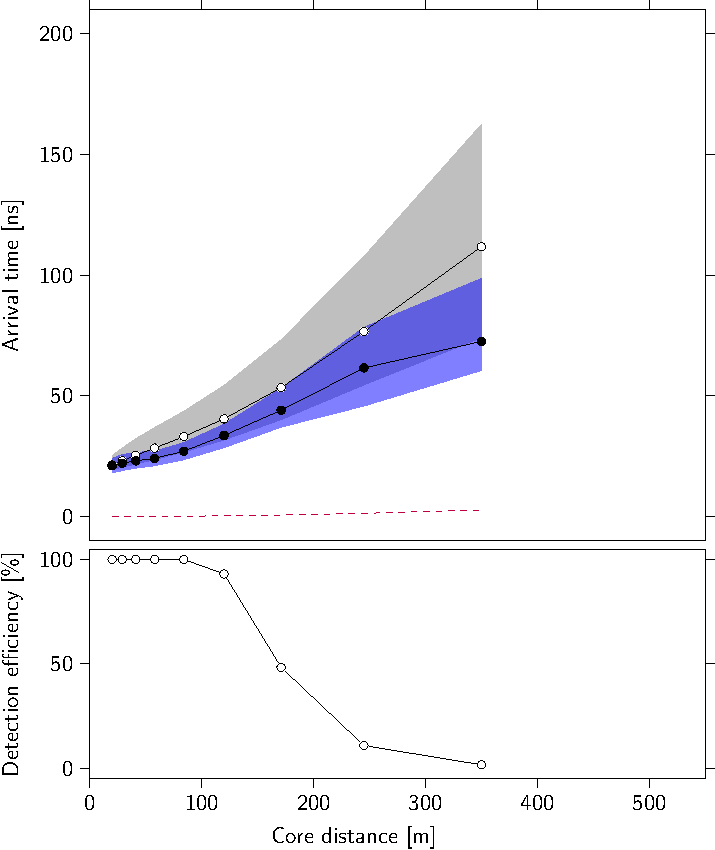
\includegraphics{plots/reconstructions/proton_E_16-0_Z_0-0_I_22_149042664_130233131}
    \caption{Compared raw shower front profile (open, gray) to detected shower profile (closed, blue). As a function of core distance the temporal distribution of leptons in the shower front is shown. The markers indicate the median arrival times, the colored bands include \SI{50}{\percent} of the particles. For the detected shower profile the arrival time of the first particle in a detector counts, if the station triggered.}
    \label{fig:shower_detected_time_profile}
\end{figure}

After combining the detected profiles from multiple showers a relation can be derrived between the time delay and core distance. For each shower energy the shower profile is fit using $t = a r ^ b$. In table [make table with fitted params] the fitted parameters are shown. This time delay is used in direction reconstruction.


\subsection{Reconstruction steps}

Raw data is first processed as described in \cref{ch:data_processing}. Because the core position is not yet known a simple direction reconstruction is performed which assumes a flat shower front. After this initial direction is determined the core position is estimated.

The shower direction can be used to improve the estimated particle density in a station by correcting for the longer path of the shower particles in the detectors, which are a factor $\cos^{-1} \theta$ higher than they would be if going vertically through the detectors. Simultaneously the effective surface of the detector is reduced by a factor $\cos \theta$. Both these effects need to be corrected for. The uncertainty in the detected density is at low particle densities dominated by Poisson statistics. The value to be considered is not the particle density but the number of detected particles. Therefore the number should be corrected for the longer path, but not the different effective area.

Using the estimated core position the direction reconstruction can use the core position to determine the radial core distance of each detector to the shower core. The reconstruction can then use non-flat shower fronts to reconstruct the core. The shape of a shower front
